\underline{Photodiode}

The final part of this experiment deals with inserting a photodiode into the circuit. It should be noted that a phototransistor is used instead of a photodiode. However, the mechanics of the devices are essentially the same in the circuit. Photodiodes have a wide depletion layer exposed to light. When light is illuminated onto the photodiode, it absorbs many photons. Photons at a high frequency excite electrons from the valence band to the conduction band since their energy level is now sufficiently higher than the bandgap energy. This allows the photodiode to be used as a means of generating electrical energy from light.
The photodiode is considered in three cases: reverse bias, zero bias, and forward bias. In the zero bias case, when electrons jump from the valence band to conduction band, the electric field in the depletion layer causes the electrons to move in a reverse-biased direction. The current is driven by these excited electrons, which as a result supply the load with power. The second case for the photodiode is reverse bias. Reverse biasing the photodiode widens the depletion layer, so that more photons can be captured. When more photons are captured, a higher current can be driven through the load. Forward biasing the photodiode decreases the size of the depletion layer, restricting the photodiode's ability to convert light into electrical energy. \\
\underline{\#9}

\centering
\begin{tabular}{| c | c | c | c |}\hline
	& V\textsubscript{in}=-5V & V\textsubscript{in}=0 & V\textsubscript{in}=5V \\\hline
	Without Flashlight & -0.01 & 0.075 & 0.82\\\hline
	With Flashlight & 0.50 & 0.52 & 0.82 \\\hline
\end{tabular}
\label{Voltage over Photodiode}
\ref{photodiode_table}
\\

\underline{\#10}
\\

Because the forward bias diode has a smaller depletion layer and thus produces less power, it is not ideal for solar cells. The reverse and no bias cases are far preferable. The photodiode should produce the most current in the reverse bias case since the wider depletion layer gives rise to a larger current. The data demonstrate that forward biasing the diode does not increase voltage over, and therefore the current through, the diode. However, the data does not illustrate a noticeable difference between the reverse bias and zero bias cases. The fact that a phototransistor and not a true photodiode is used might partly explain why the results are slightly different from what is expected. Given the data, the zero bias case is preferable. This is because an external source must reverse bias the photodiode, thereby consuming electrical power in the process. The no bias case generates roughly the same amount of power in the experiment and does not require any power from an external source for biasing.
In most applications, this may not necessarily hold. Moreover, increasing the reverse bias voltage may help the photodiode to begin to absorb much more light energy. Another possible issue could be that the depletion region of the "photodiode" used is already quite wide, and biasing it does not widen it much more. As a result, the effect of biasing is not noticeable.
The voltage over the diodes increases when the light is on in both the reverse and no bias cases. The reason it does not in the forward bias case is because forward biasing the diode decreases the size of the depletion region, making it so that it cannot absorb as much light.

\begin{figure}[h!]
	\centering
	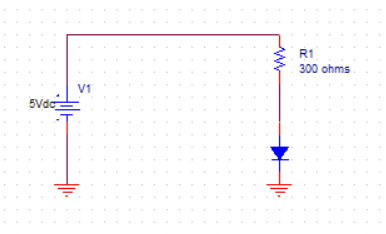
\includegraphics{CircuitSchematic.PNG}
	\caption{Experiment 4 Circuit}
	\label{fig:Circuit_Pic}
\end{figure}
